%%%%%%%%%%%%%%%%%%%%%%%%%%%%%%%%%%%%%%%%%%%%%%%%%%%%%%%%%%%%%%%%%%%%%%
% Overleaf (WriteLaTeX) Example: Molecular Chemistry Presentation
%
% Source: http://www.overleaf.com
%
% In these slides we show how Overleaf can be used with standard 
% chemistry packages to easily create professional presentations.
% 
% Feel free to distribute this example, but please keep the referral
% to overleaf.com
% 
%%%%%%%%%%%%%%%%%%%%%%%%%%%%%%%%%%%%%%%%%%%%%%%%%%%%%%%%%%%%%%%%%%%%%%

\documentclass{beamer}

\mode<presentation>
{
  \usetheme{Madrid}       % or try default, Darmstadt, Warsaw, ...
  \usecolortheme{default} % or try albatross, beaver, crane, ...
  \usefonttheme{default}    % or try default, structurebold, ...
  \setbeamertemplate{navigation symbols}{}
  \setbeamertemplate{caption}[numbered]
} 

\usepackage[english]{babel}
\usepackage[utf8x]{inputenc}
\usepackage{chemfig}
\usepackage[version=3]{mhchem}

\usepackage{hyperref}
  \hypersetup{colorlinks=true}
  \hypersetup{urlcolor=blue}
  \hypersetup{linkcolor = .}
\usepackage{xcolor}
\usepackage{siunitx}
  \sisetup{separate-uncertainty = true}
\usepackage{physics}
\usepackage[font=small,labelfont=bf]{caption}
\usepackage{subcaption}
\usepackage[en-GB]{datetime2}
\usepackage{feynmp}
\DeclareGraphicsRule{*}{mps}{*}{}

\usepackage{scalerel}
\newcommand{\mylbrace}[2]{\vspace{#2pt}\hspace{6pt}\scaleleftright[\dimexpr5pt+#1\dimexpr0.06pt]{\lbrace}{\rule[\dimexpr2pt-#1\dimexpr0.5pt]{-4pt}{#1pt}}{.}}
\newcommand{\myrbrace}[2]{\vspace{#2pt}\scaleleftright[\dimexpr5pt+#1\dimexpr0.06pt]{.}{\rule[\dimexpr2pt-#1\dimexpr0.5pt]{-4pt}{#1pt}}{\rbrace}\hspace{6pt}}

% Here's where the presentation starts, with the info for the title slide
\title[BESIII Oxford]{BESIII Oxford Group Meeting}
\author{Martin Tat}
\institute{Oxford LHCb}
\date{\today}

\titlegraphic{
\includegraphics[width = 5cm, height = 3.8cm]{lhcb.jpg}\hspace{1cm}~%
              
\includegraphics[width = 5cm, height = 3.8cm]{bes3.jpg}}

\begin{document}

\begin{frame}
  \titlepage
\end{frame}

% These three lines create an automatically generated table of contents.
%\begin{frame}{Outline}
%  \tableofcontents
%\end{frame}

\section{Intorduction}
\begin{frame}{Introduction}
  \begin{itemize}
    \setlength\itemsep{2em}
    \item{$D\to K^+K^-\pi^+\pi^-$ analysis}
    \item{Previously: Fit to $\Delta E$ and $m_\text{BC}$ to get ST yield in MC}
    \item{Current progress:}
    \begin{itemize}
      \item{Finished code for all tag modes}
      \item{Run over all MC and data}
      \item{Studied $KK\pi\pi$ single tag backgrounds}
    \end{itemize}
    \item{Tag modes:}
    \begin{itemize}
      \item{Flavour: $K\pi$, $K\pi\pi^0$, $K\pi\pi\pi$, $Ke\nu$}
      \item{CP even: $KK$, $\pi\pi$, $KS\pi^0\pi^0$, $K_L\pi^0$, $K_L\omega$, $\pi\pi\pi^0$}
      \item{CP odd: $K_S\pi^0$, $K_S\eta(\gamma\gamma, \pi\pi\pi^0)$, $K_S\omega$, $K_S\eta'(\pi\pi\eta, \pi\pi\gamma)$, $K_S\phi$, $K_L\pi^0\pi^0$}
      \item{CP conjugate: $K_S\pi\pi$, $KK\pi\pi$}
    \end{itemize}
  \end{itemize}
\end{frame}

\begin{frame}{MC samples}
  \centering
  \begin{tabular}{ccc}
    MC sample & Events ($10^6$) & Luminosity scale ($2010$/$2011$) \\
    \hline
    $D^0\bar{D^0}$     & $74$   & $21.8$/$21.8$ \\
    $D^+D^-$           & $29$   & $10.9$/$10.8$ \\
    $q\bar{q}$         & $122$  & $7.8$/$7.3$   \\
    $\psi(2S)\gamma$   & $34$   & $10.8$/$10.1$ \\
    $J/\psi\gamma$     & $22$   & $10.8$/$10.1$ \\
    $\tau\tau$         & $60$   & $10.8$/$10.1$ \\
    non-$D\bar{D}$     & $10$   & $10.8$/$10.1$ \\ \\ \\
  \end{tabular}
  \begin{itemize}
    \item{Did not run over $ee$ and $\mu\mu$ MC}
  \end{itemize}
\end{frame}

\section{$\Delta E$ fit in data vs MC}
\begin{frame}{$\Delta E$ fit in data vs MC}
  \begin{figure}
    \centering
    \begin{subfigure}{0.5\textwidth}
      \centering
      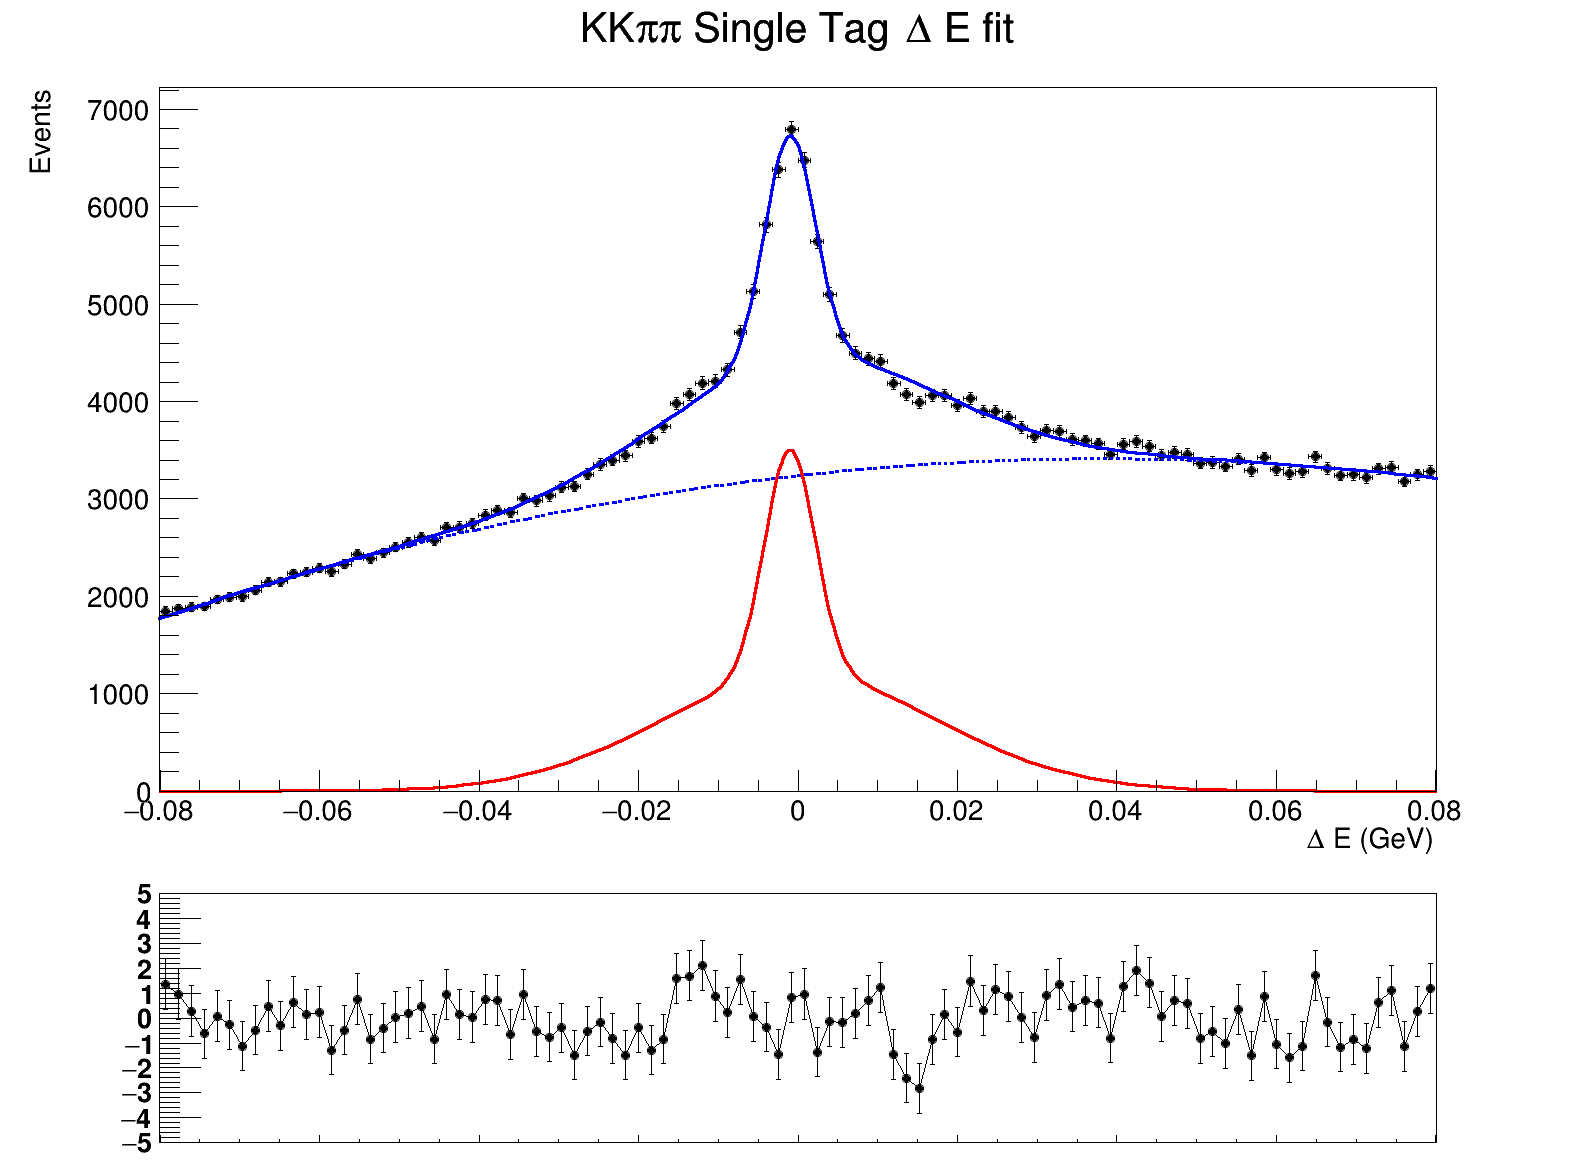
\includegraphics[width=\textwidth]{KKpipiSingleTagPlot.png}
      \caption{$\Delta E$, data}
    \end{subfigure}%
    \begin{subfigure}{0.5\textwidth}
      \centering
      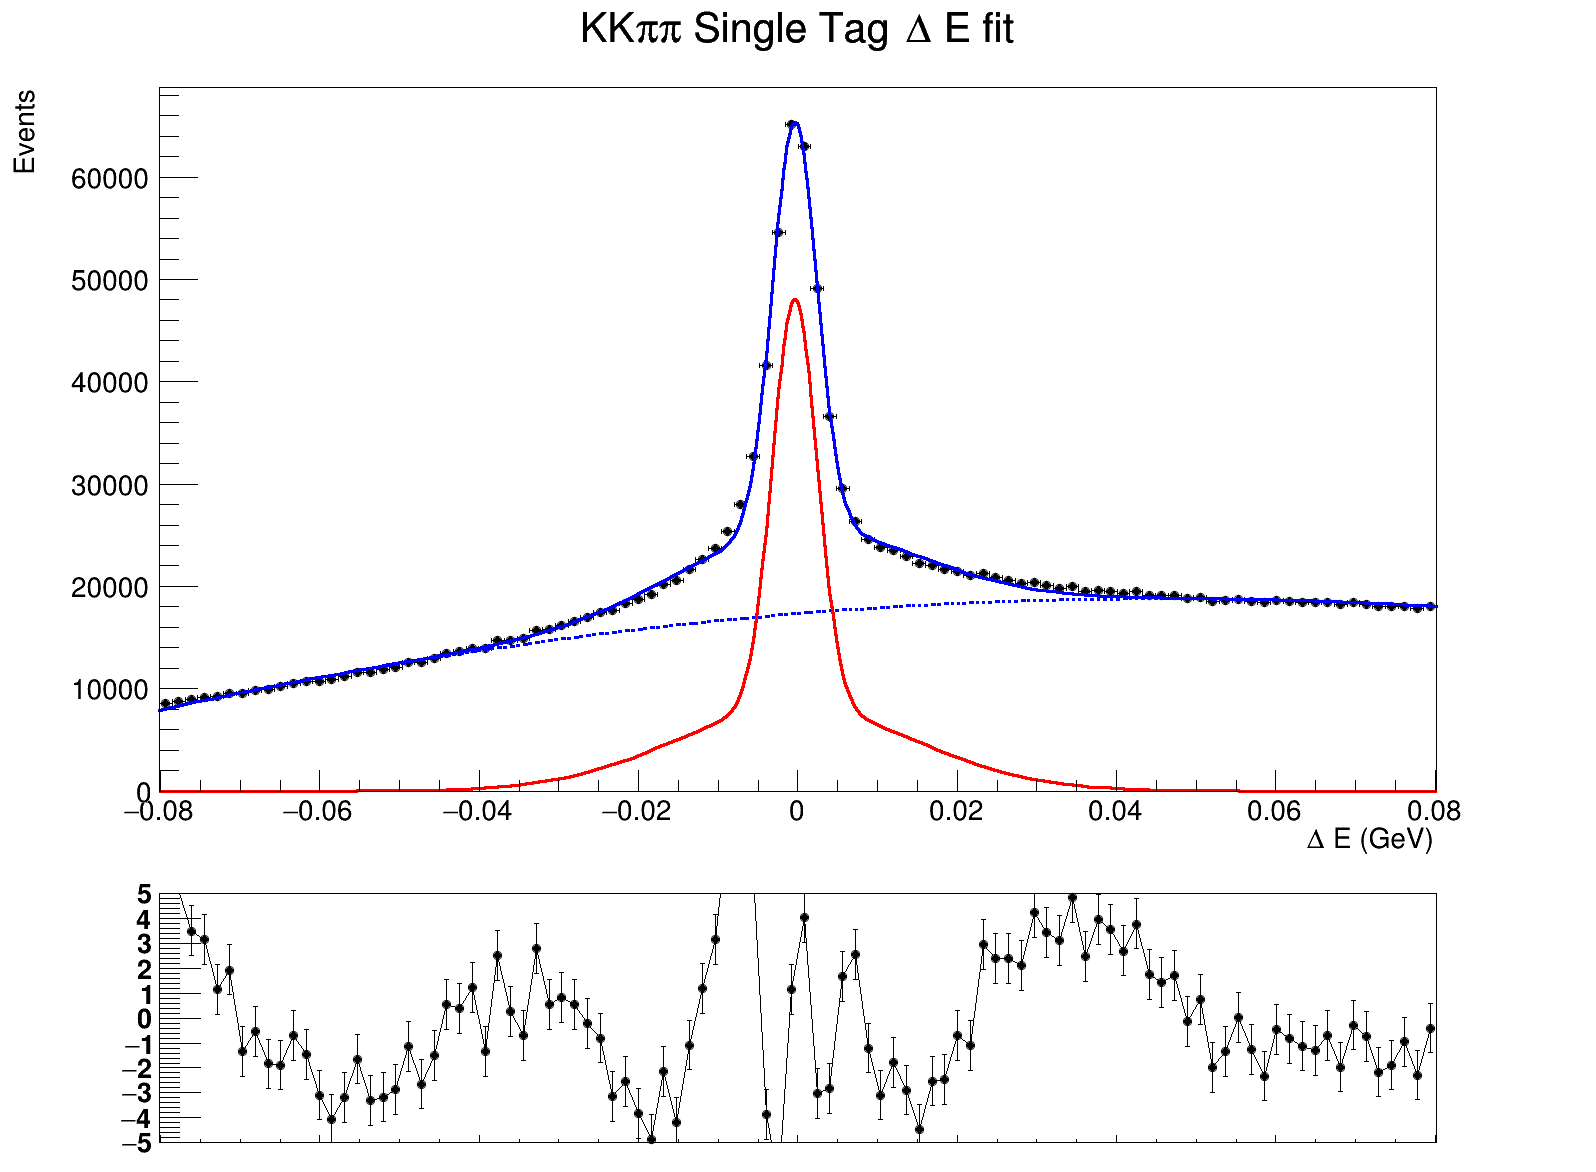
\includegraphics[width=\textwidth]{KKpipiSingleTagDeltaEPlot.png}
      \caption{$\Delta E$, MC}
    \end{subfigure}
  \end{figure}
  Why are the MC pulls wrong? \\
  Does $\Delta E$ for data look sensible?
\end{frame}

\section{$KK\pi\pi$ single tag backgrounds}
\begin{frame}{$KK\pi\pi$ single tag backgrounds}
  \begin{figure}
    \centering
    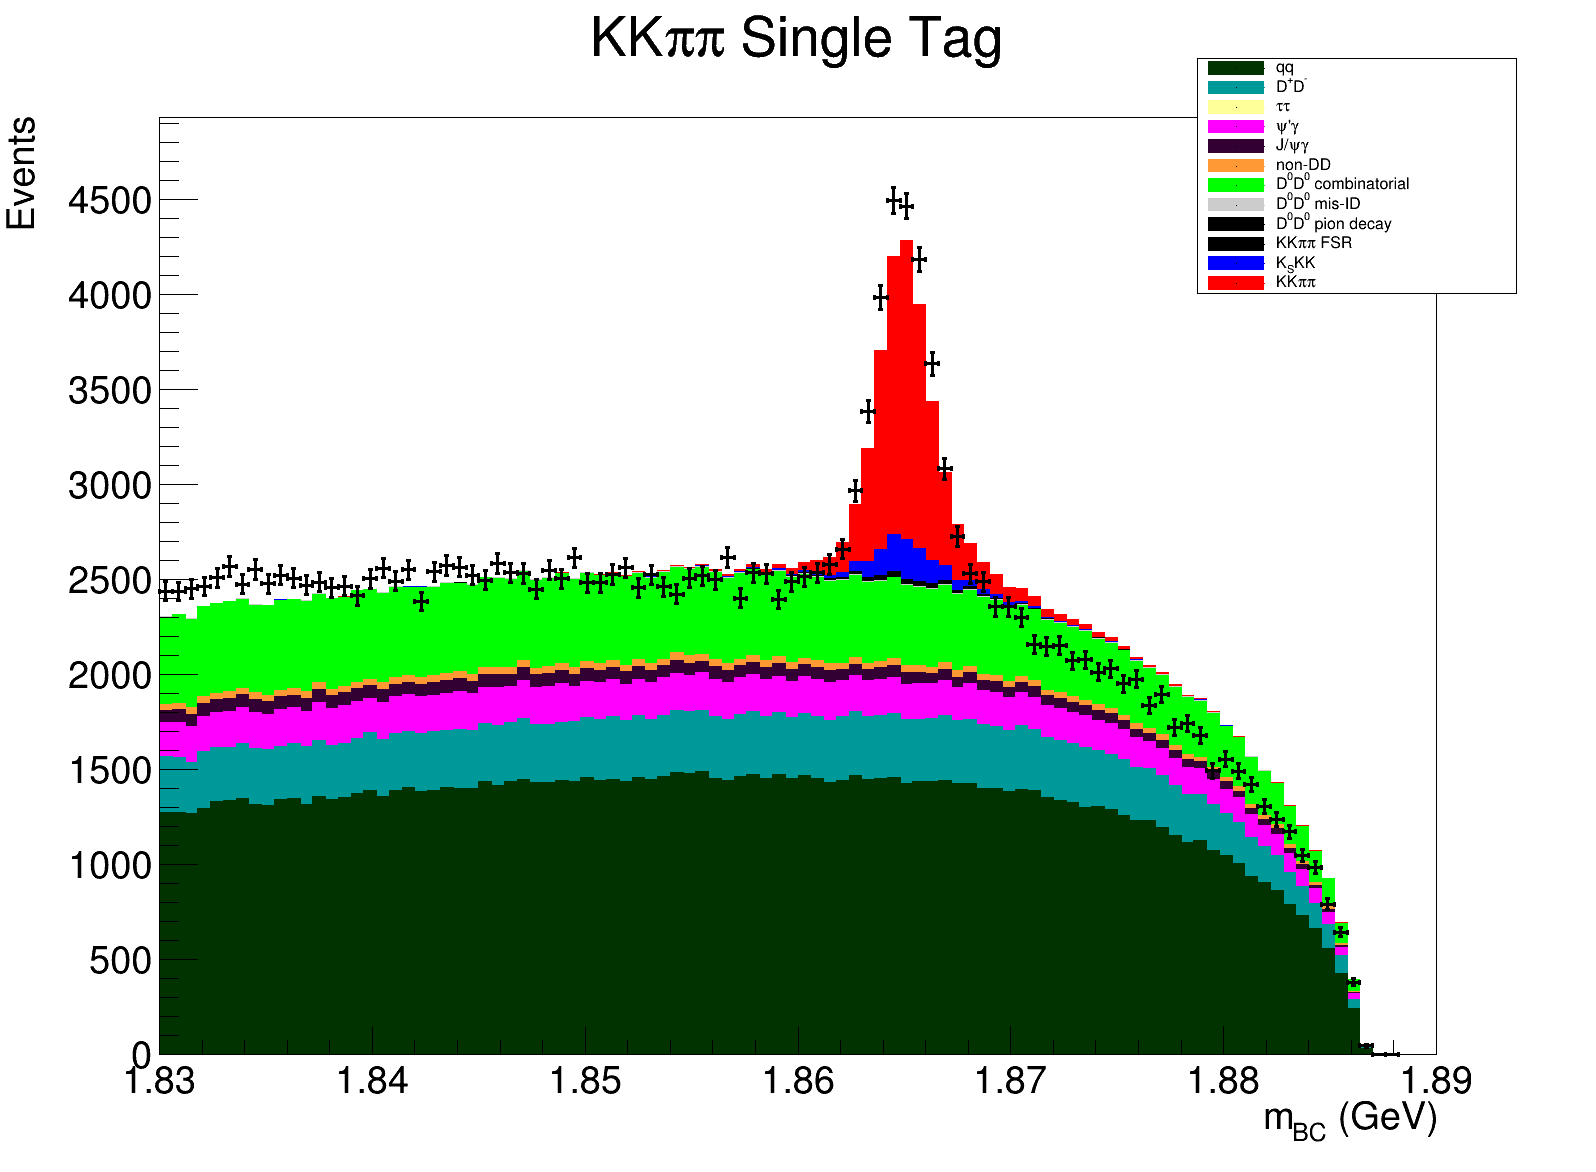
\includegraphics[width=0.8\textwidth]{MCPlusData.png}
    \caption{$KK\pi\pi$ single tag $m_\text{BC}$ components}
  \end{figure}
  Should I be worried that data doesn't match MC?
\end{frame}

\section{Next steps}
\begin{frame}{Next steps}
  \begin{itemize}
    \setlength\itemsep{2em}
    \item{Account for peaking backgrounds with Gaussian and fit for ST yields}
    \item{Study backgrounds for all other modes}
    \item{Start with DT yields, check with expectation from amplitude model}
  \end{itemize}
\end{frame}

\end{document}
